\section{Architecture of distributed systems}

This section introduces and analyzes common design patterns of distributed
systems. It is divided into two subsections based on
CAP-theorem\cite{gilbert2002brewer} that states that no distributed system can
achieve consistency, availability and partition tolerance at the same time. Due
the nature of distributed systems network partitions are bound to happen, thus
designers of distributed system need to choose whether the system remains
available during the partition or keeps the data consistent.

\subsection{CP-systems}

\begin{figure}[h!]
  \centering
    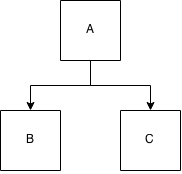
\includegraphics{pictures/cp_system.png}
  \caption{CP-system with a single master node and two slaves}
\label{cpimage}
\end{figure}

CP-systems endorse data consistency over availability. In practice this means
that when a network between two or more database nodes malfunctions, the
system should stop handling both, read and write requests from clients and wait
until the network is healed. Failure to do so might bring the systems into an
inconsistent state, where nodes of the system have different view of the same
datum. Consider figure~\ref{cpimage} that shows a CP-system consisting of a
single master node \(A\) and two slaves \(B\) and \(C\). Clients are able to
read from all of the nodes, but only node \(A\) accepts writes. After a
successful write, \(A\) replicates the write to the slave nodes. If the
connection between \(A\) and \(B\) fails, the system is partitioned into two
sets, one containing \(A\) and \(C\), and other containing only \(B\). Now if
the client first writes a new document to \(A\) and then tries to read it from
both \(B\) and \(C\), what happens is that \(C\) correctly returns the written
document, but \(B\) reports that the document can not be found. This happens
because master \(A\) was not able to replicate the new write to node \(B\)
because the network between the nodes was down. Because now \(B\) and \(C\) have
a different view of the same datum, the system can not be considered as
CP-system anymore. The situation can be fixed by not accepting a write from the
client, when the master node detects that it is not able to replicate the writes
to all nodes. 

As in the example, a common way to model CP-systems is a master/slave
architecture, where one node at a time acts as a master and other nodes are
slaves. To achieve consistency, only master is able to accept write requests and
depending on the architecture, slaves might be able to accept read requests. If
slaves handle the read requests, the distributed system might not be consistent
at all times. For example, node \(A\) accepted a write but did not had time to
replicate it to node \(B\) when it replies to the read request accessing that
object, the database would incorrectly report that object is not found. However
after \(A\) has replicated the object to \(B\) the database is again in
consistent state. This is called eventual consistency.

Vogels specifies eventual consistency as a specific form of weak
consistency\cite{vogels2009eventually}. A system with weak consistency does not
guarantee that subsequent accesses to the updated object always returns the
updated object but a set of conditions need to be met before. The period between
when the object is updated and when it is guaranteed is called
\emph{inconsistency window}.

In eventual consistency, the system guarantees that if no new updates are made
to the object, eventually all access will return the updated object. In this
case, the maximum inconsistency window in best case scenario can be calculated
from different factors of the system, such as communication delay between nodes
and the load of the system. Of course in exceptional events such as network
partition the inconsistency window can grow as large as the event occur.

The problem that many CP-systems face is what happens when the master node
becomes unavailable. That may occur for many reasons, for example the node can
suffer from hardware failure or the network between master and other nodes goes
down. Naturally the system needs to be able to recover from such cases and many
different procedures have been developed to cope with the problem. Next we
discuss how Raft consensus algorithm handles election of a new leader.

Raft is a consensus algorithm developed to replace more complex algorithm Paxos.
Raft aims to be more understandable and better uncoupled than its
predecessor\cite{chiefari1998living}. Consensus algorithms allow collection of
services to agree on some state even when some of them fails. They often arise
in context of \emph{replicated state machines}, where each service compute
identical copies of the same data. To achieve consistency, Raft selects a
distinguished leader which has a complete responsibility of managing the
replicated log and replicating them to other services. When the leader fails or
becomes unavailable, the new leader must be elected.

Raft detects leader failures with heartbeats. Each node starts as a follower and
remains in that state as long as it receives heartbeat signals from the leader.
If a follower receives no heartbeat in a period of time called \emph{election
timeout}, it assumes there are no leader and begins the leader election.

In the beginning of leader election, the follower that received no heartbeat
promotes itself to a candidate and sends vote request messages to the other
clients. A client grants the vote for the first candidate requesting the vote
and declines the rest. The candidate continues in this state until one of the
three things things happens:

\begin{enumerate}
  \item The candidate wins the election and promotes itself to the leader if it
  receives votes from majority of the cluster. Once the candidate wins the
  election it starts sending heartbeats to the other nodes and establishes the
  authority and prevents new elections.
  \item While waiting for the votes, the candidate might receive a heartbeat
  from other node. In this case it demotes itself to the follower state and
  recognizes the new leader.
  \item Last outcome is that the candidate does not win or lose the elections.
  If many followers become candidates at the same time, it is possible that none
  of the candidates receive majority of votes and initiate a new round of
  vote requests. Raft uses randomized election time outs to ensure that no two
  clients are candidates indefinitely. Another candidate might still be waiting
  out the time out when other candidate receives a majority of the votes and
  starts sending heartbeats and ending elections.
\end{enumerate}

The actual leader election in RAFT is a bit more complicated than described
above, having a concept of \emph{terms} to measure time as a logical clocks, but
they were left out for clarity. The original paper explains the election in more
detail and the website of Raft
algorithm\footnote{\url{https://raftconsensus.github.io/}} has an excellent
interactive visualization about the leader election.

\subsection{AP-systems}

\missingfigure{AP-system}
